\titre{Chemin :} Un chemin dans un graphe $G=(S,A)$ est une séquence de sommets $C = [ c_1,\ldots,c_n ]$ telle que $(c_i,c_{i+1}) \in A \forall i \in \{ 1 .. n-1 \}$ \\
 
\titre{Longueur :} La longueur de $C$ est $n-1$ \\

\titre{Chemin simple :} $i\neq j \impl c_i \neq c_j$ \\

\titre{Cycle :} Un cycle est un chemin "simple" mais avec $c_1 = c_n$, sauf les chemins du type $[u,v,u]$ des graphes non orientés. \\

\titre{Critère d'isomorphie :} Deux graphes isomorphes ont le même nombre de cycles de chaque longueur. Ce critère est nécessaire mais non suffisant. (fig6)\\

\titre{Condition nécessaire :} \\
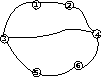
\includegraphics[width=100px]{Images/fig4.pdf} \hspace{1cm} 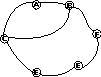
\includegraphics[width=100px]{Images/fig5.pdf} \\

\titre{Condition non suffisante :} \\

\includegraphics[width=100px]{Images/fig6.pdf} \\

\titre{Composante connexe :} Soit $G=(S,A)$ un graphe non orienté. Une commposante connexe de $G$ est un sous ensemble maximal de sommets $S'$ tel que pour toute paire de sommets $(u,v)$ de $S'$, il existe un chemin de $u$ à $v$. \\

\titre{Connexité :} Un graphe est dit connexe s'il ne contient qu'une seule composante connexe. \\

\titre{Composante fortement connexe :} Soit $G=(S,A)$ un graphe orienté. Une commposante fortement connexe de $G$ est un sous ensemble maximal de sommets $S'$ tel que pour toute paire de sommets $(u,v)$ de $S'$, il existe un chemin de $u$ à $v$. \\

\titre{Graphe fortement connexe :} Ses sommets forment une composante fortement connexe. \\

